\begin{frame}
	\frametitle{Señales básicas: Exponencial Compleja}\centering
    \begin{itemize}
        \item \alert{Continua:} $x(t)=A\mathsf{e}^{\:j\omega t}$
		\begin{itemize}
            \item \color{blue}$x(t)=x(t+T)$\color{black}, con $T=\frac{1}{f}=\frac{2\pi}{\omega}$ \\
            \color{cyan}{\tiny $x(t+T)=A\mathsf{e}^{\:j\omega (t+\frac{2\pi}{\omega})}=A\mathsf{e}^{\:j(\omega t+2\pi)}=A\mathsf{e}^{\:j\omega t}\mathsf{e}^{\:j2\pi}=A\mathsf{e}^{\:j\omega t}$=x(t)}\color{black}
            \vspace{0.1cm}
            \item \color{blue}$\omega=2\pi f$ \color{black}es la frecuencia ($\omega$ rad/s, $f$ Hz)
            \vspace{0.1cm}
            \item \color{blue}$\omega_1\neq\omega_2 \Rightarrow x_1(t)\neq x_2(t)$\color{black}, para $0<\omega<\infty$
            \vspace{0.1cm}
        \end{itemize}
    \end{itemize}
    \begin{minipage}{0.25\textwidth}
        \centering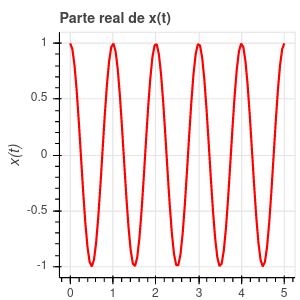
\includegraphics[width=\textwidth]{Figuras/exp_real.png}
    \end{minipage}
    \begin{minipage}{0.25\textwidth}
        \centering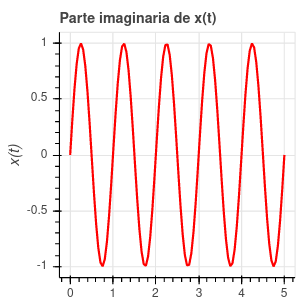
\includegraphics[width=\textwidth]{Figuras/exp_imag.png}
    \end{minipage}

    \begin{block}{{\scriptsize Fórmula de Euler}}\centering
        \scriptsize{$e^{j(\omega t+\phi)}=cos(\omega t+\phi)+j sin(\omega t+\phi)\Rightarrow \left\lbrace\begin{matrix}
            cos(\omega t+\phi)=\frac{e^{j(\omega t+\phi)}+e^{-j(\omega t+\phi)}}{2}\\
            sin(\omega t+\phi)=\frac{e^{j(\omega t+\phi)}-e^{-j(\omega t+\phi)}}{2j}\\
        \end{matrix}\right.$}
    \end{block}
\end{frame}


\begin{frame}
	\frametitle{Señales básicas: Exponencial Compleja}\centering

	\begin{itemize}
		\item \alert{Continua (Forma General):} $x(t)=C \mathsf{e}^{a t}$, con $C,a\in\mathbb{C}$
		\vspace{0.1cm}
		\begin{itemize}{\small
            \item $\left.\begin{matrix}C=|C|\mathsf{e}^{j\phi}\\a=r+j\omega\end{matrix}\right\rbrace \Rightarrow \color{blue}x(t)=|C| \mathsf{e}^{r t}\mathsf{e}^{\:j(\omega t+\phi)}\color{black}$
    %        \vspace{0.1cm}
            \item Sinusoidal multiplicada por exponencial
            \vspace{0.1cm}
            \item Decreciente ($r<0$), constante ($r=0$) o creciente ($r>0$)
            \vspace{0.1cm}
        }\end{itemize}
    \end{itemize}
    \begin{minipage}{0.25\textwidth}
        \centering\scriptsize{$r<0$}\\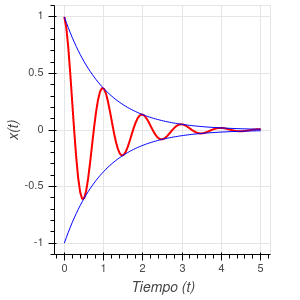
\includegraphics[width=\textwidth]{Figuras/exp_decreciente.png}
    \end{minipage}
    \begin{minipage}{0.25\textwidth}
        \centering\scriptsize{$r=0$}\\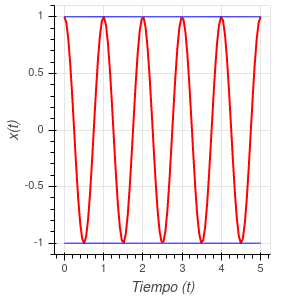
\includegraphics[width=\textwidth]{Figuras/exp_sin.png}
    \end{minipage}
    \begin{minipage}{0.25\textwidth}
        \centering\scriptsize{$r>0$}\\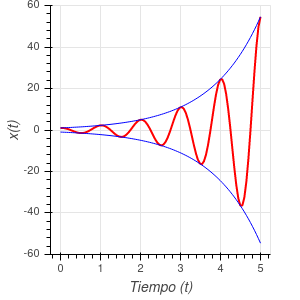
\includegraphics[width=\textwidth]{Figuras/exp_creciente.png}        
    \end{minipage}
    \begin{block}{{\scriptsize Fórmula de Euler}}\centering
        \scriptsize{$e^{j(\omega t+\phi)}=cos(\omega t+\phi)+j sin(\omega t+\phi)\Rightarrow \left\lbrace\begin{matrix}
            cos(\omega t+\phi)=\frac{e^{j(\omega t+\phi)}+e^{-j(\omega t+\phi)}}{2}\\
            sin(\omega t+\phi)=\frac{e^{j(\omega t+\phi)}-e^{-j(\omega t+\phi)}}{2j}\\
        \end{matrix}\right.$}
    \end{block}
\end{frame}


\begin{frame}
	\frametitle{Señales básicas: Exponencial Compleja}\centering
    \begin{itemize}
        \vspace{0.1cm}
		\item \alert{Discreta:} $x[n]=C \mathsf{e}^{j\omega n}$
		\begin{itemize}{\small
            \item \color{blue}$\omega=2\pi f$~\color{black} es la frecuencia en rad/muestra
            \vspace{0.1cm}
            \item \color{blue}$x[n]=x[n+N]$\color{black}, con $N=\frac{1}{f}=\frac{2\pi}{\omega}$ \color{red}sólo si \color{black}
            \vspace{0.1cm}
            \color{cyan}{\tiny $x[n+N]=C\mathsf{e}^{\:j\omega (n+N)}=C\mathsf{e}^{\:j(\omega n+\omega N)}=C\mathsf{e}^{\:j\omega n}\mathsf{e}^{\:j\omega N}=x[n]$\\
            \vspace{0.1cm}
            $\mathsf{e}^{\:j\omega N}=1\Rightarrow 2\pi f N=2\pi k \Rightarrow f=\frac{k}{N}$, para algún $N,k\in\mathbb{N}$\\
            Nota: $\frac{k}{N}$ es una fracción irreducible, en caso contrario $\frac{a}{b}=\frac{m\cdot k}{m\cdot N}=\frac{k}{N}$
            }\color{black}


            \vspace{0.1cm}
            \item \color{blue}$\omega_1\neq\omega_2 \Rightarrow x_1[n]\neq x_2[n]$\color{black}, \color{red}sólo para $0<\omega<2\pi\color{black}$\\
            \vspace{0.1cm}
            \color{cyan}{\scriptsize $\omega_k=\omega+2\pi k \Rightarrow$
            $C\mathsf{e}^{\:j(\omega + 2\pi k) n}=C\mathsf{e}^{\:j\omega n+j2\pi k n}=C\mathsf{e}^{\:j\omega n}\mathsf{e}^{\:j2\pi k n}=C\mathsf{e}^{\:j\omega n}$}\color{black}
            \vspace{0.1cm}
        }\end{itemize}
    \end{itemize}

    \begin{block}{{\scriptsize Fórmula de Euler}}
        \centering
        \scriptsize{$e^{j\omega n+\phi}=cos(\omega n+\phi)+j sin(\omega n+\phi)\Rightarrow \left\lbrace\begin{matrix}
            cos(\omega n+\phi)=\frac{e^{j(\omega n+\phi)}+e^{-j(\omega n+\phi)}}{2}\\
            sin(\omega n+\phi)=\frac{e^{j(\omega n+\phi)}-e^{-j(\omega n+\phi)}}{2j}\\
        \end{matrix}\right.$}
    \end{block}
\end{frame}


\begin{frame}
	\frametitle{Señales básicas: Exponencial Compleja}\centering
    \begin{itemize}{\scriptsize
        \vspace{0.1cm}
		\item \alert{Exponencial Discreta (sinusoidal):} $x[n]=C \alpha^n$, con $C,\alpha\in\mathbb{C}$
		\begin{itemize}{\scriptsize
            \item $\left.\begin{matrix}C=|C|e^{\phi}\\\alpha=|\alpha|e^{j\omega}\end{matrix}\right\rbrace \Rightarrow\color{blue}x(t)=|C||\alpha|^{n}e^{~j\omega n+\phi}\color{black}$
            \vspace{0.1cm}
            \item Decreciente ($0<\alpha<1$), constante ($\alpha=1$), o creciente ($\alpha>1$)
            \vspace{0.1cm}
        }\end{itemize}
    }\end{itemize}
    \begin{minipage}{0.25\textwidth}
        \centering\scriptsize{$0<|\alpha|<1$}\\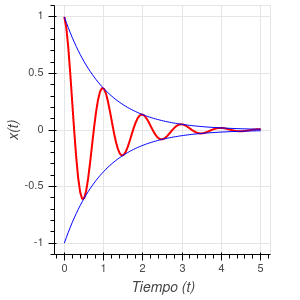
\includegraphics[width=\textwidth]{Figuras/exp_decreciente.png}
    \end{minipage}
    \begin{minipage}{0.25\textwidth}
        \centering\scriptsize{$|\alpha|=1$}\\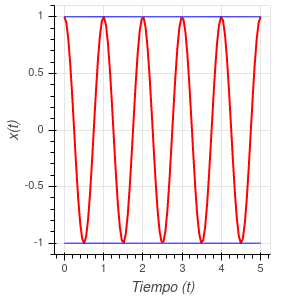
\includegraphics[width=\textwidth]{Figuras/exp_sin.png}
    \end{minipage}
    \begin{minipage}{0.25\textwidth}
        \centering\scriptsize{$|\alpha|>1$}\\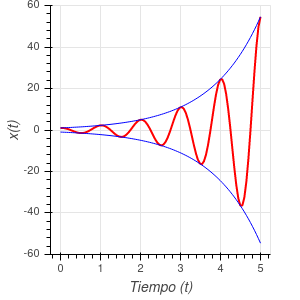
\includegraphics[width=\textwidth]{Figuras/exp_creciente.png}
    \end{minipage}

    \begin{block}{Fórmula de Euler}
        \centering
        \scriptsize{$e^{j\omega n+\phi}=cos(\omega n+\phi)+j sin(\omega n+\phi)\Rightarrow \begin{matrix}
            cos(\omega n+\phi)=\frac{e^{j\omega n+\phi}+e^{-j\omega n-\phi}}{2}\\
            sin(\omega n+\phi)=\frac{e^{j\omega n+\phi}-e^{-j\omega n-\phi}}{2}\\
        \end{matrix}$}
    \end{block}
\end{frame}

%%%%%%%%%%%%%%%%%%%%%%%%%%%%%%%%%%%%%%%%%%%%%%

\begin{frame}
	\frametitle{Señales básicas: Impulso}
	
	\begin{itemize}
        \item \alert{Continuo ($\delta$ de Dirac):} {\scriptsize \hspace{1cm}$\delta(t)=\left \{ \begin{array}{l} \infty \:\: \: \:t=0\\0 \:\: \:\: \forall t \neq0\end{array}\right .$}%
        \begin{columns}[c]
            \begin{column}{0.2\textwidth}\centering
                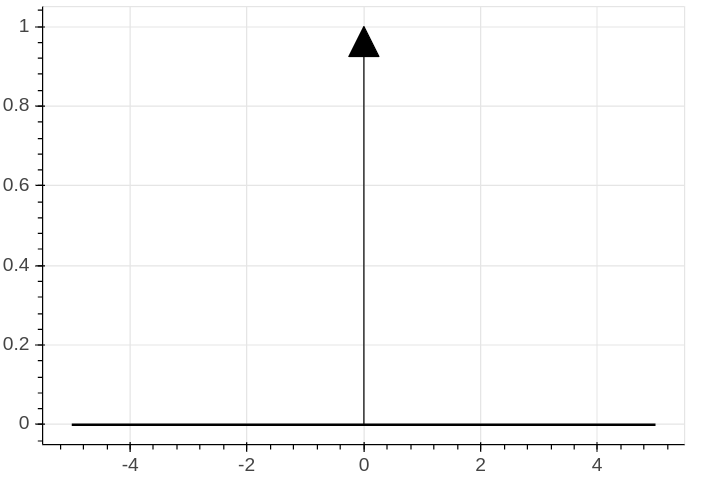
\includegraphics[width=4cm]{./Figuras/dirac}\\%
            \end{column}
            \hspace{0.3cm}
            \begin{column}{0.65\textwidth}
                {\scriptsize
                \begin{itemize}
                    {\scriptsize
                    \vspace{0.1cm}
                    \item Es un funcional:\\ \vspace{0.1cm}
                    $\int_{-\infty}^{\infty} f(t)\delta(t)dt=f(0)$\hspace{0.2cm}\color{olivegreen}$\int_{-\infty}^{\infty} f(t)\delta(t-t_0)dt=f(t_0)$\color{black}\\
                    \item Algunas propiedades:
                    $\int_{t_1}^{t_2} f(t)\delta(t-t_0)dt=\left\{\! \!\begin{array}{l}f(t_0)  \:\:\: t_1\!<t_0\!<t_2 \\ 0 \:\:\: c.c.    \end{array}\right .$
                    $\forall a\neq 0 \Rightarrow \delta(at)=\frac{\delta(t)}{|a|}$
                    $(x \ast \delta)(t) = \int_{-\infty}^\infty x(\tau)\delta(t-\tau)d\tau=x(t)$\\
                }\end{itemize}
                \vspace{0.2cm}
                \vspace{0.2cm}
            }\end{column}
        \end{columns}
        \vspace{-0.4cm}
        \item \alert{Discreto ($\delta$ de Kronecker):} {\scriptsize \hspace{0.5cm}$\delta(n)=\left \{ \begin{array}{l} 1\:\: \: \:n=0\\0 \:\: \:\: \forall n \neq0\end{array}\right .$}
        \begin{columns}[c]
            \begin{column}{0.22\textwidth}{\scriptsize
                \centering
                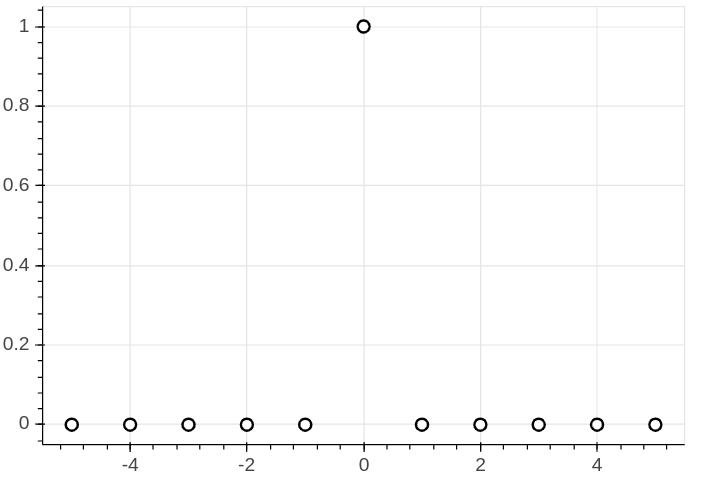
\includegraphics[width=4cm]{./Figuras/kronecker}\\%
            }\end{column}
            \begin{column}{0.65\textwidth}{\scriptsize
                \hspace{1.5cm}\color{olivegreen}$x[n]=\sum_{k=-\infty}^{\infty} x[k]\delta[k-n]$\color{black}\\
                \vspace{0.4cm}
                \hspace{1.5cm}$(x\! \ast\! \delta)[n] \!=\! \sum_{k=-\infty}^\infty x[k]\delta[n-k]=x[n]$
            }\end{column}
        \end{columns}
    \end{itemize}
\end{frame}
	
%%%%%%%%%%%%%%%%%%%%%%%%%%%%%%%%%%%%%%%%%%%%%%

\begin{frame}
\frametitle{Señales básicas: Escalón unitario}

\begin{itemize}

\begin{columns}[c]
    \begin{column}{7.0cm}
    
    \item \alert{Continuo:} $u(t)=\left \{ \begin{array}{l} 0 \:\: \: \:t<0\\1 \:\: \:\:  t \ge 0\end{array}\right .$

\vspace{0.1cm}

    
    \small Relación con el impulso:

\vspace{0.1cm}

$\delta(t)=\frac{du(t)}{dt}$

\vspace{0.1cm}

$u(t)=\int _{-\infty} ^t \delta(\tau)d\tau$

\vspace{0.1cm}

Convolución: $(x \ast u)(t)=\int _{-\infty} ^t x(\tau)d\tau $
    
    \end{column}
\hspace{-2.5cm}\begin{column}{5cm}
    \begin{figure}
\centering
\footnotesize
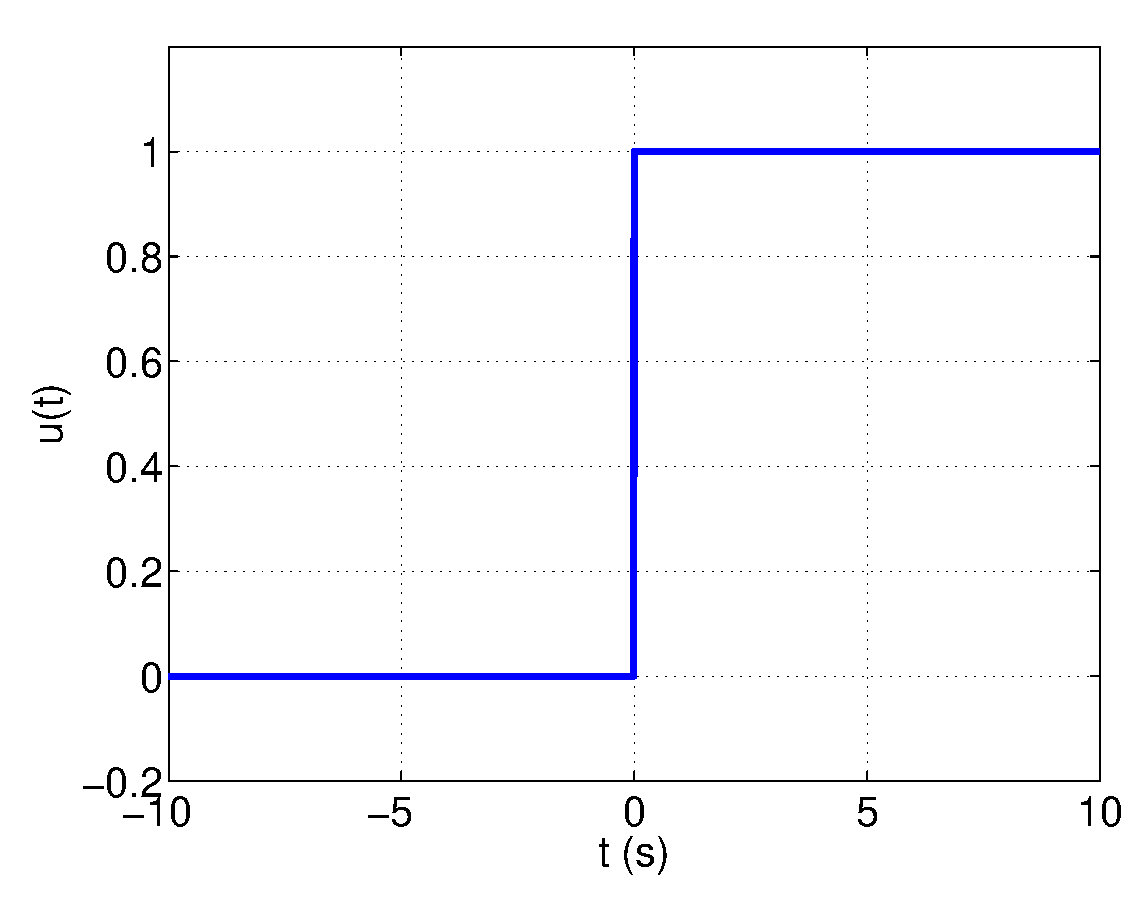
\includegraphics[width=4cm]{./Figuras/EscalonT.eps} 
\end{figure}
    \end{column}
    \end{columns}
    
\vspace{-0.2cm}

\hspace{1cm}\begin{columns}[c]
    \begin{column}{6.0cm}
                    \item \alert{Discreto:}  $u[n]=\left \{ \begin{array}{l} 0\:\: \: \:n<0\\1 \:\: \:\:  n \ge 0\end{array}\right .$
    
            \vspace{0.2cm}
    
    \small Relación con el impulso:

\vspace{0.2cm}

$\delta[n]=u[n]-u[n-1]$

\vspace{0.2cm}

$u[n]=\sum _{k=-\infty} ^n \delta[k]$
    
    \vspace{0.2cm}

Convolución: $(x\! \ast \! u)[n]\!=\!\sum _{k=-\infty} ^n x[k]$
    
    \end{column}
\hspace{-1.5cm}\begin{column}{5cm}
    \begin{figure}
\centering
\footnotesize
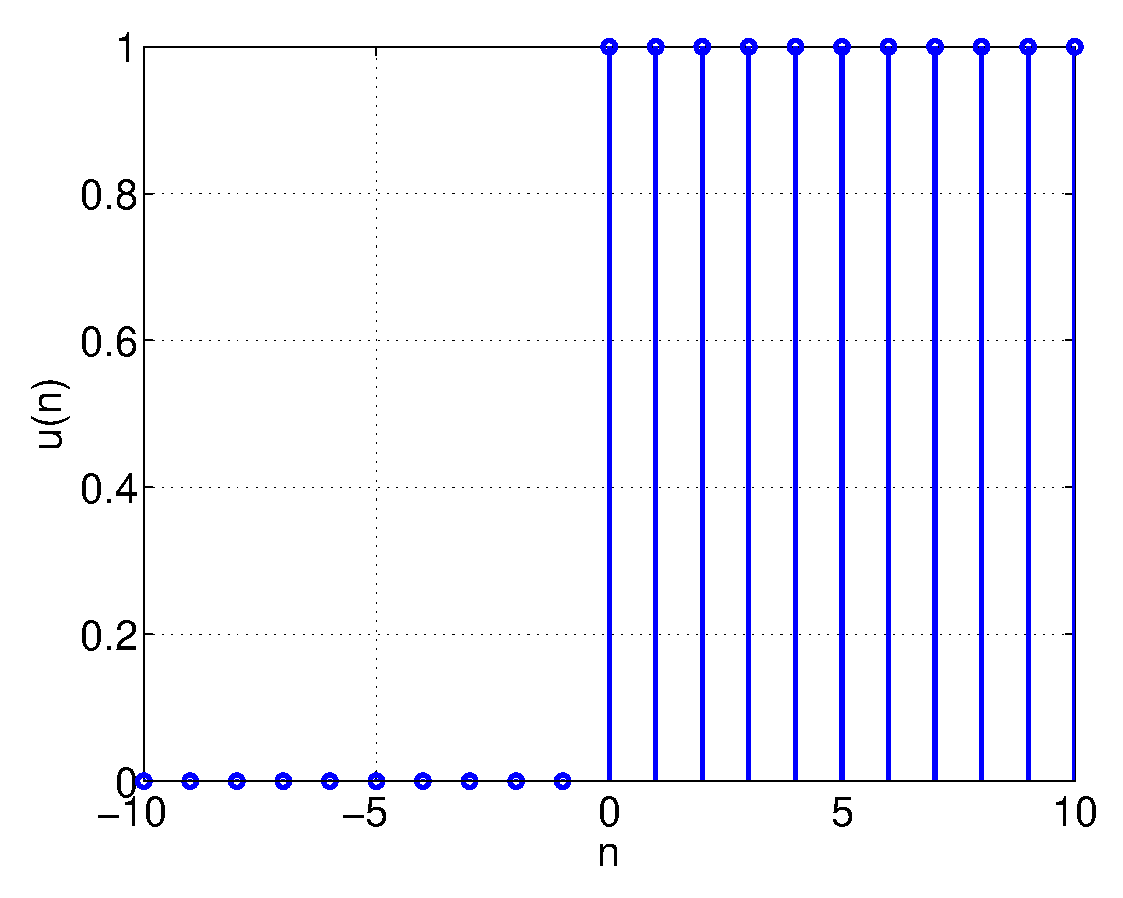
\includegraphics[width=4cm]{./Figuras/EscalonN.eps} 
\end{figure}
    \end{column}
    \end{columns}


\end{itemize}

\small El producto de cualquier señal $x(\cdot)$ por $u(\cdot)$ produce una señal causal.

\end{frame}

%%%%%%%%%%%%%%%%%%%%%%%%%%%%%%%%%%%%%%%%%%%%%%%
	
	
\begin{frame}
\frametitle{Señales básicas: Rampa}

\begin{itemize}

\begin{columns}[c]
    \begin{column}{7.0cm}
        \item \alert{Continuo:} $r(t)=\left \{ \begin{array}{l} 0 \\ t \end{array}\begin{array}{l}t<0 \\ t \ge 0\end{array}\right .$

\vspace{0.1cm}

    
    \small Relación con el escalón:

\vspace{0.1cm}

$u(t)=\frac{dr(t)}{dt}$

\vspace{0.1cm}

$r(t)=\int _{-\infty} ^t u(\tau)d\tau$

\vspace{0.1cm}

    
    \end{column}
\hspace{-2.5cm}\begin{column}{5cm}
    \begin{figure}
\centering
\footnotesize
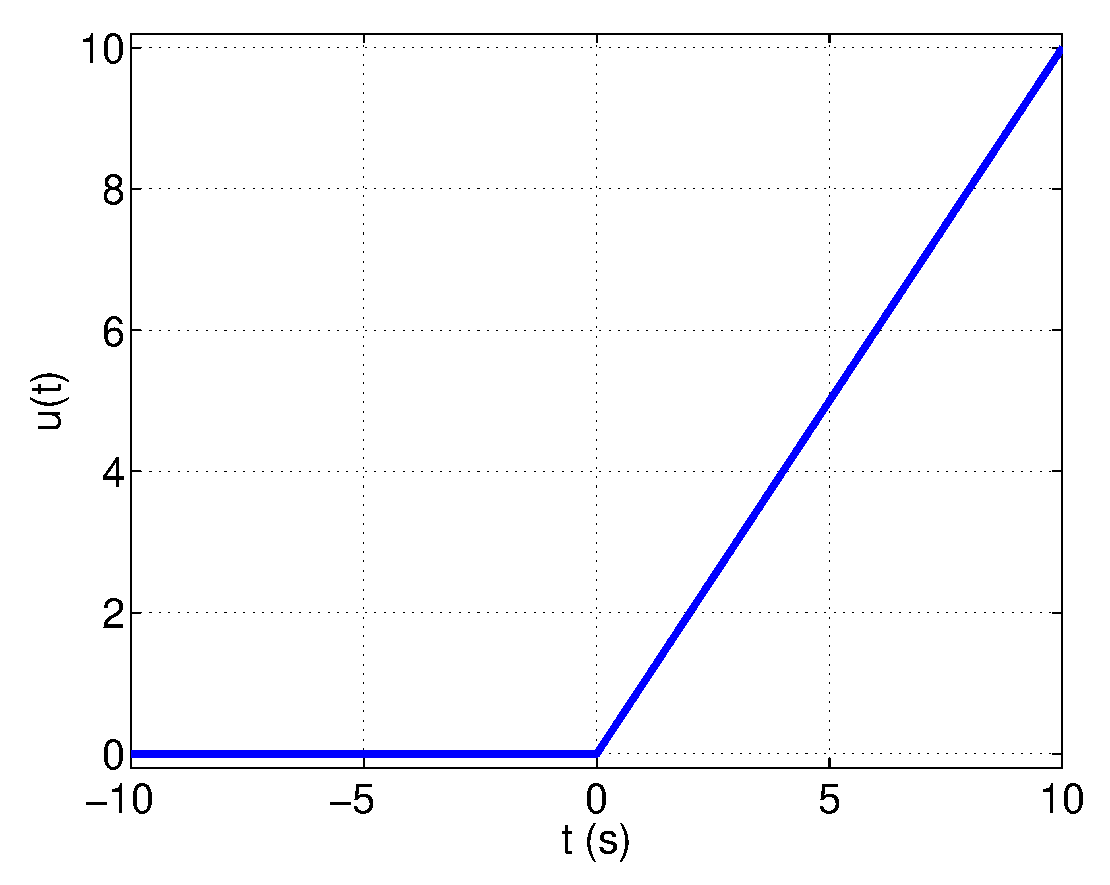
\includegraphics[width=4cm]{./Figuras/RampaT.eps} 
\end{figure}
    \end{column}
    \end{columns}
    
\vspace{-0.2cm}

\hspace{1cm}\begin{columns}[c]
    \begin{column}{6.0cm}
                    \item \alert{Discreto:}  $r[n]=\left \{ \begin{array}{l} 0 \\n+1\end{array}\begin{array}{l} n<0\\n \ge 0\end{array}\right .$
    
    
            \vspace{0.2cm}
    
    \small Relación con el escalón:

\vspace{0.2cm}

$u[n]=r[n]-r[n-1]$

\vspace{0.2cm}

$r[n]=\sum _{k=-\infty} ^n u[k]$
    
    \vspace{0.2cm}
    
    \end{column}
\hspace{-1.5cm}\begin{column}{5cm}
    \begin{figure}
\centering
\footnotesize
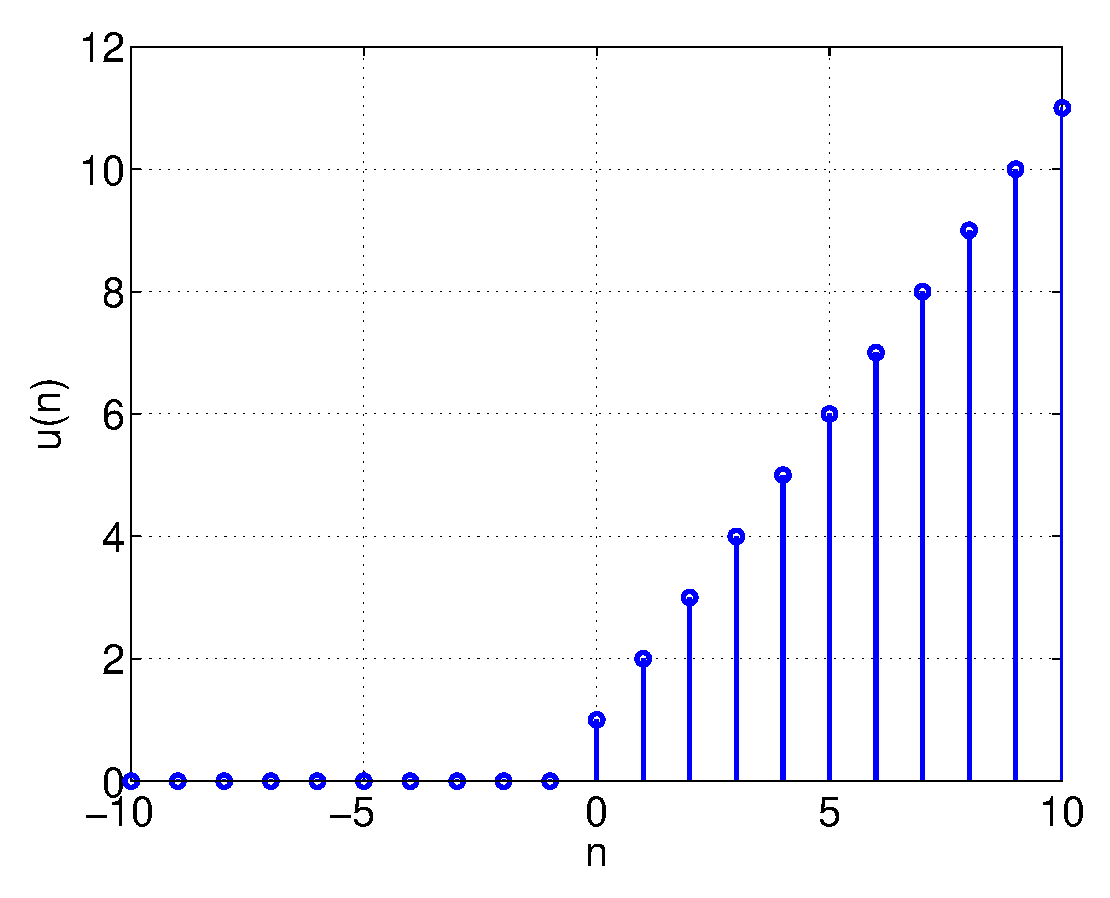
\includegraphics[width=4cm]{./Figuras/RampaN.eps} 
\end{figure}
    \end{column}
    \end{columns}


\end{itemize}


\end{frame}


%%%%%%%%%%%%%%%%%%%%%%%%%%%%%%%%%%%%%%%%%%%%%%

\begin{frame}\frametitle{Señales básicas: Pulsos}

    \begin{itemize}
        \begin{columns}[c]
            \begin{column}{5cm}
            \item \alert{Pulso rectangular}
                \vspace{0.3cm}
                $\Pi(t)=\left \{ \begin{array}{l} 1 \:\: \: \:|t| \le \frac{1}{2}\\0 \:\: \:\:  |t| > \frac{1}{2}\end{array}\right .$            
                \begin{figure}
                    \centering
                    \footnotesize
                    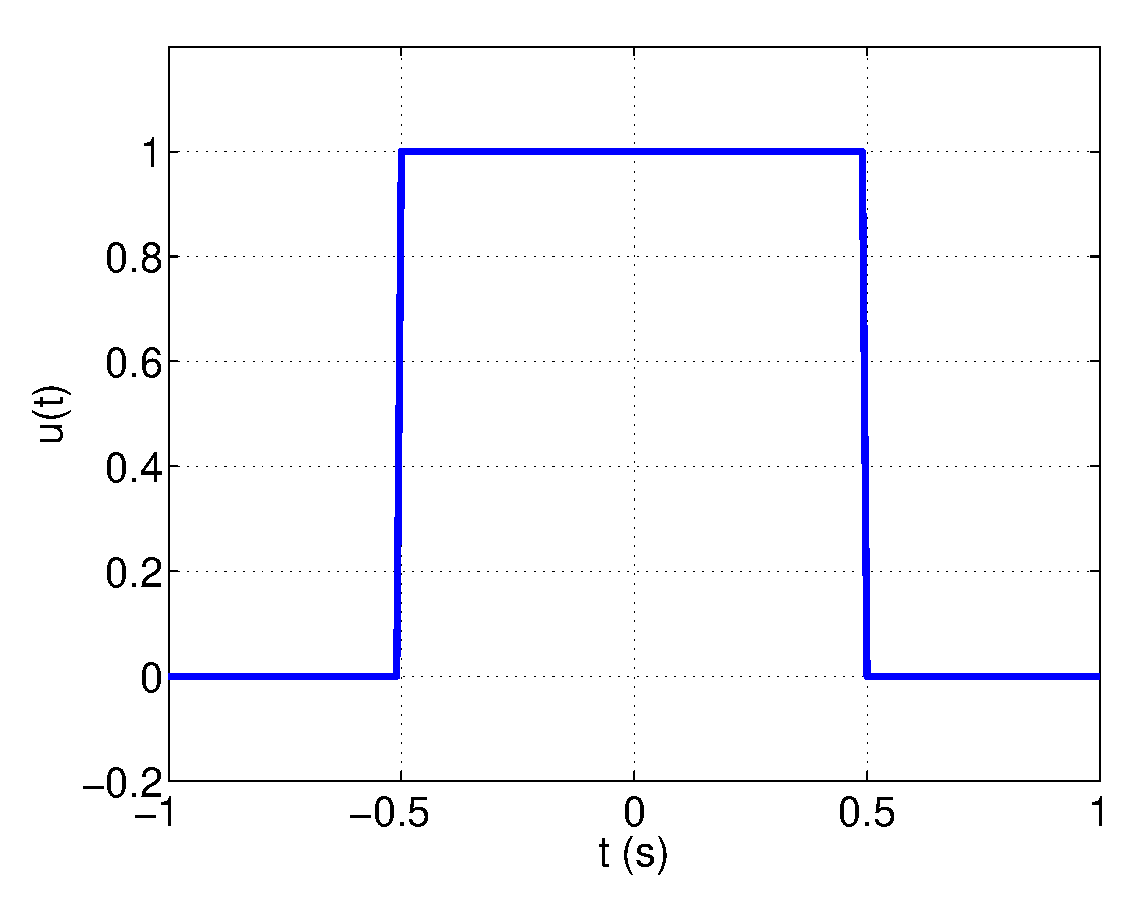
\includegraphics[width=5cm]{./Figuras/PulsoRect.eps} 
                \end{figure}
            \end{column}
            \begin{column}{5.cm}
                \item \alert{Pulso triangular}
                \vspace{0.3cm}
                $\Lambda(t)=\left \{\!\! \begin{array}{l} t+1 \:\: \: \:-1 \le t \le 0\\1-t \:\: \:\: \:\: \:\: \: 0 \le t \le 1\end{array}\right .$            
                \begin{figure}
                    \centering
                    \footnotesize
                    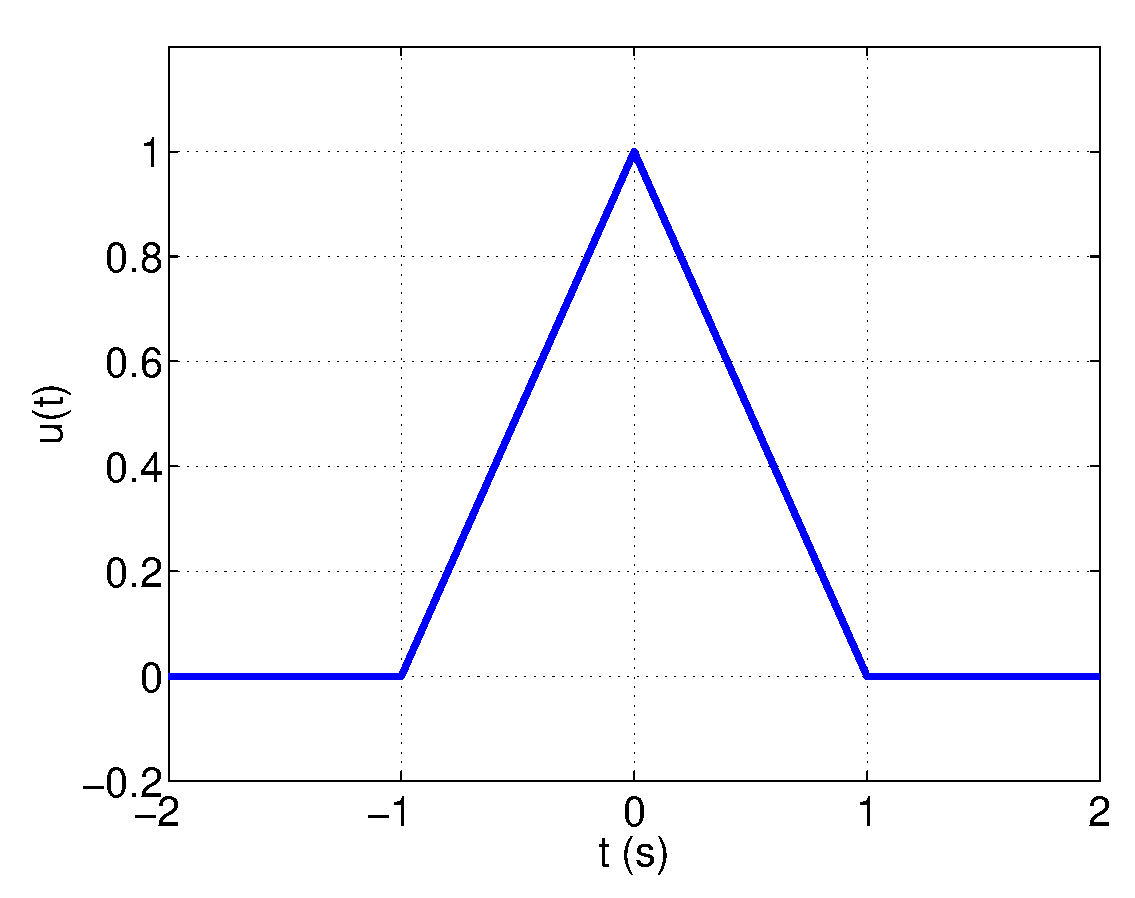
\includegraphics[width=5cm]{./Figuras/PulsoTri.eps} 
                \end{figure}
            \end{column}
        \end{columns}
    \end{itemize}
\end{frame}

%%%%%%%%%%%%%%%%%%%%%%%%%%%%%%%%%%%%%%%%%%%%%%%%%%%%%%


\begin{frame}
\frametitle{Señales básicas: muestreo, sinc, signo }

\vspace{-0.4cm}

\begin{itemize}



\begin{columns}[c]
    \begin{column}{4.5cm}
    
    \vspace{-0.8cm}
    
    \item \alert{Muestreo}

\vspace{0.3cm}

        $Sa(t)=\left \{ \begin{array}{l} \frac{sin(t)}{t} \:\: \: \:t \neq 0\\1 \:\: \:\: \:\: \:\: \:\: \:t=0\end{array}\right .$
        
            \item \alert{Sinc}

\vspace{0.3cm}

        $sinc(t)=\left \{\!\! \begin{array}{l} \frac{sin(\pi t)}{\pi t} \:\: \: \: t \ne 0 \\1 \:\: \:\:  \:\: \:\: \:\: \:\:  \: t=0\end{array}\right .$
    
    
    \vspace{0.7cm}
    
    
    \item \alert{Signo}

\vspace{0.3cm}

        $sgn(t)=\left \{\!\! \begin{array}{l} 1 \:\: \: \: \:\: \:\:t > 0 \\-1 \:\: \:\:   t<0 \\ 0  \:\: \:\:  \:\: \:\: t=0\end{array}\right .$


    
    \end{column}
\hspace{-0.5cm}	\begin{column}{4.5cm}
    
    \vspace{0.6cm}
            \begin{figure}
\centering
\footnotesize
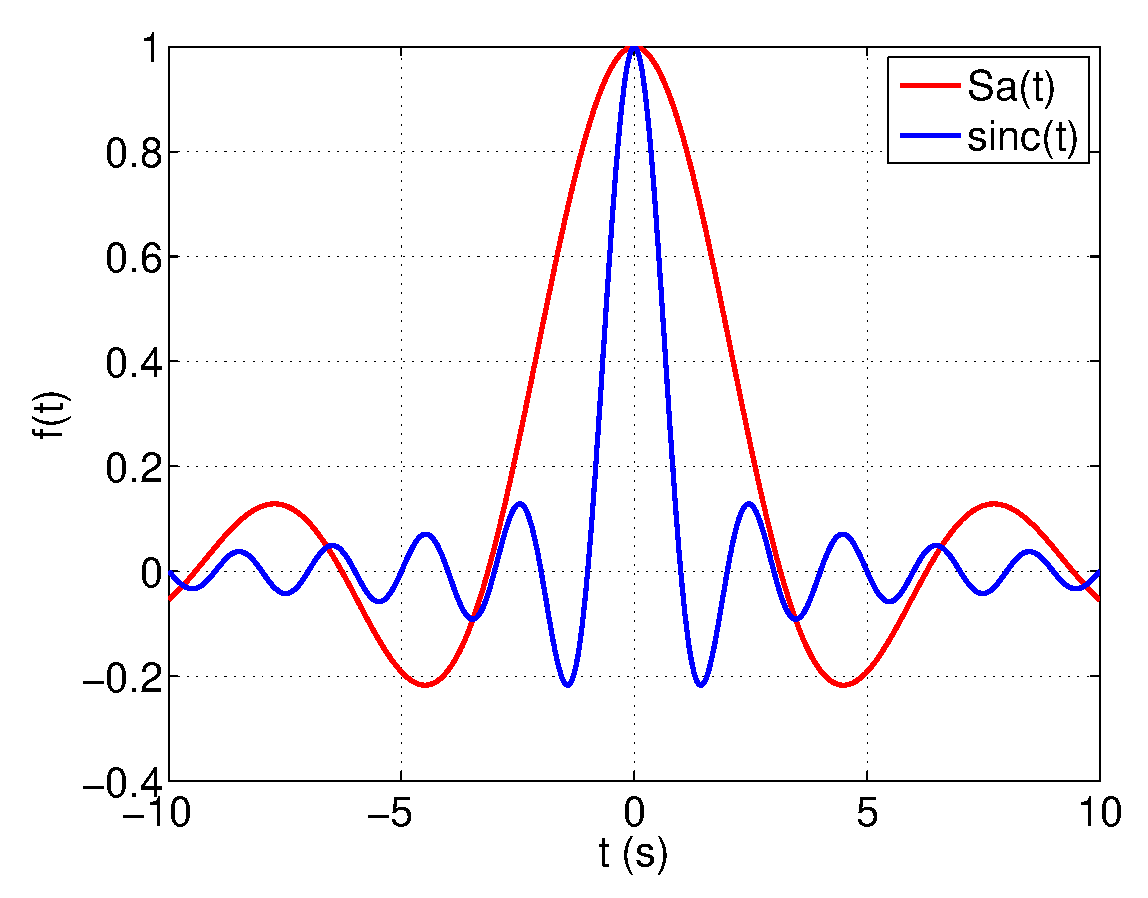
\includegraphics[width=4.5cm]{./Figuras/MuestreoSinc.eps} 
\end{figure}

            \begin{figure}
\centering
\footnotesize
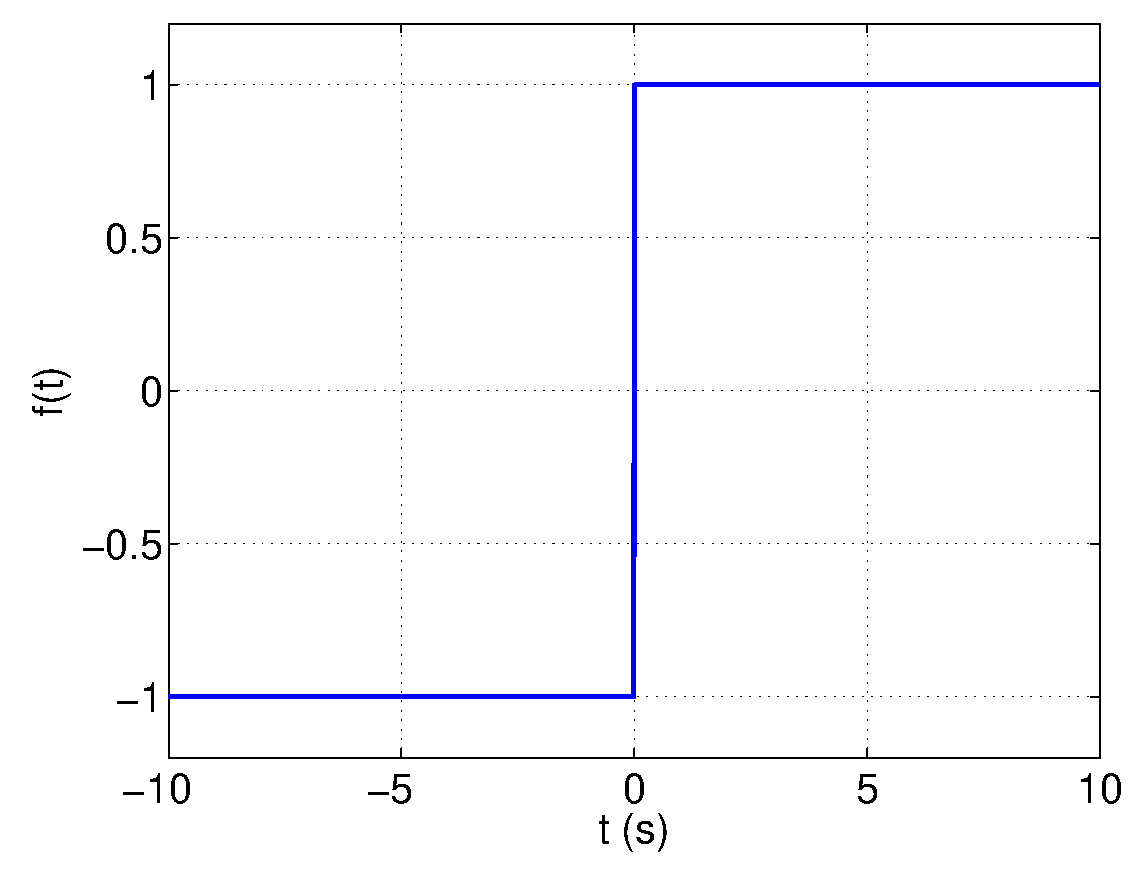
\includegraphics[width=4.5cm]{./Figuras/Signo.eps} 
\end{figure}

    
    \end{column}
    \end{columns}


\end{itemize}





\end{frame}

%%%%%%%%%%%%%%%%%%%%%%%%%%%%

\begin{frame}
\frametitle{Señales básicas: ondas  }

\begin{itemize}

\begin{columns}[c]
    \begin{column}{4.5cm}
    
    \item \alert{Onda cuadrada}

\vspace{0.3cm}

    
            
            \begin{figure}
\centering
\footnotesize
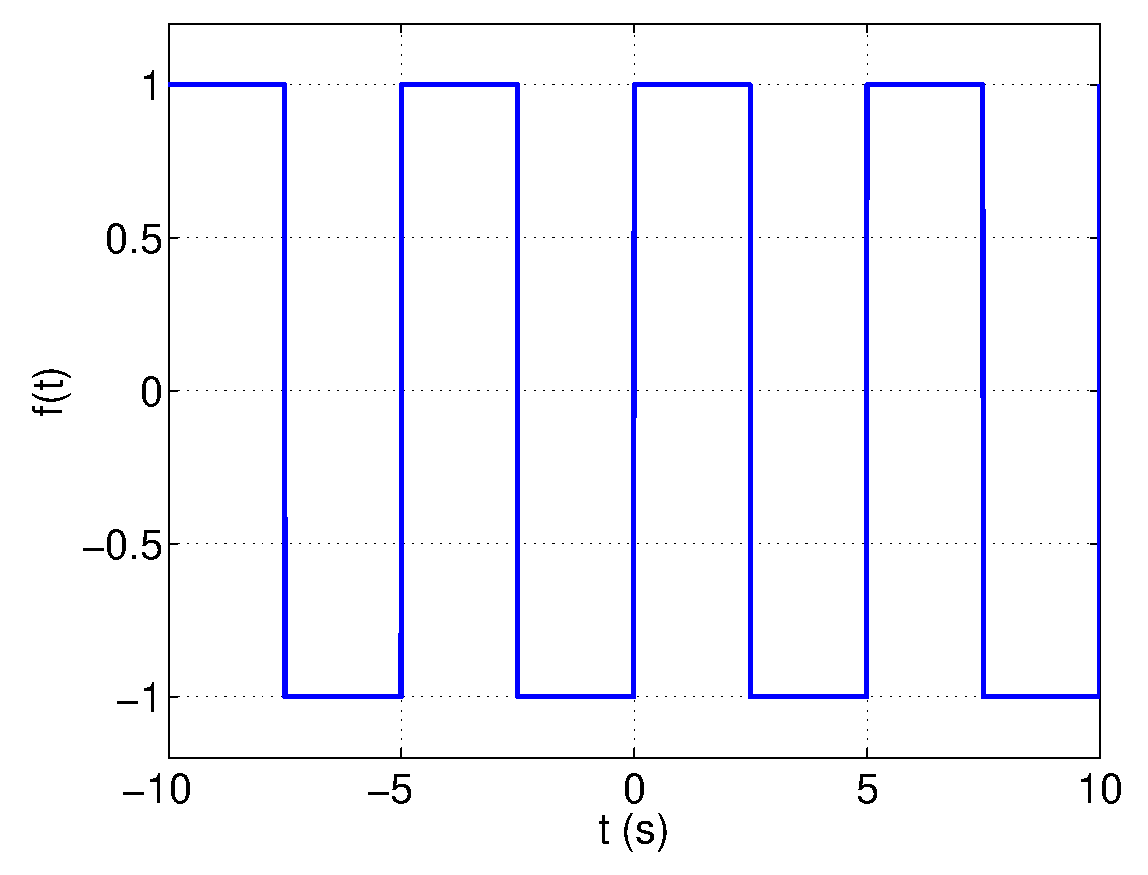
\includegraphics[width=4.5cm]{./Figuras/Square.eps} 

$T=5$
\end{figure}
    
    
    

    
    \end{column}
\hspace{-0.5cm}	\begin{column}{4.5cm}
    
        \item \alert{Onda triangular}

\vspace{0.3cm}




            \begin{figure}
\centering
\footnotesize
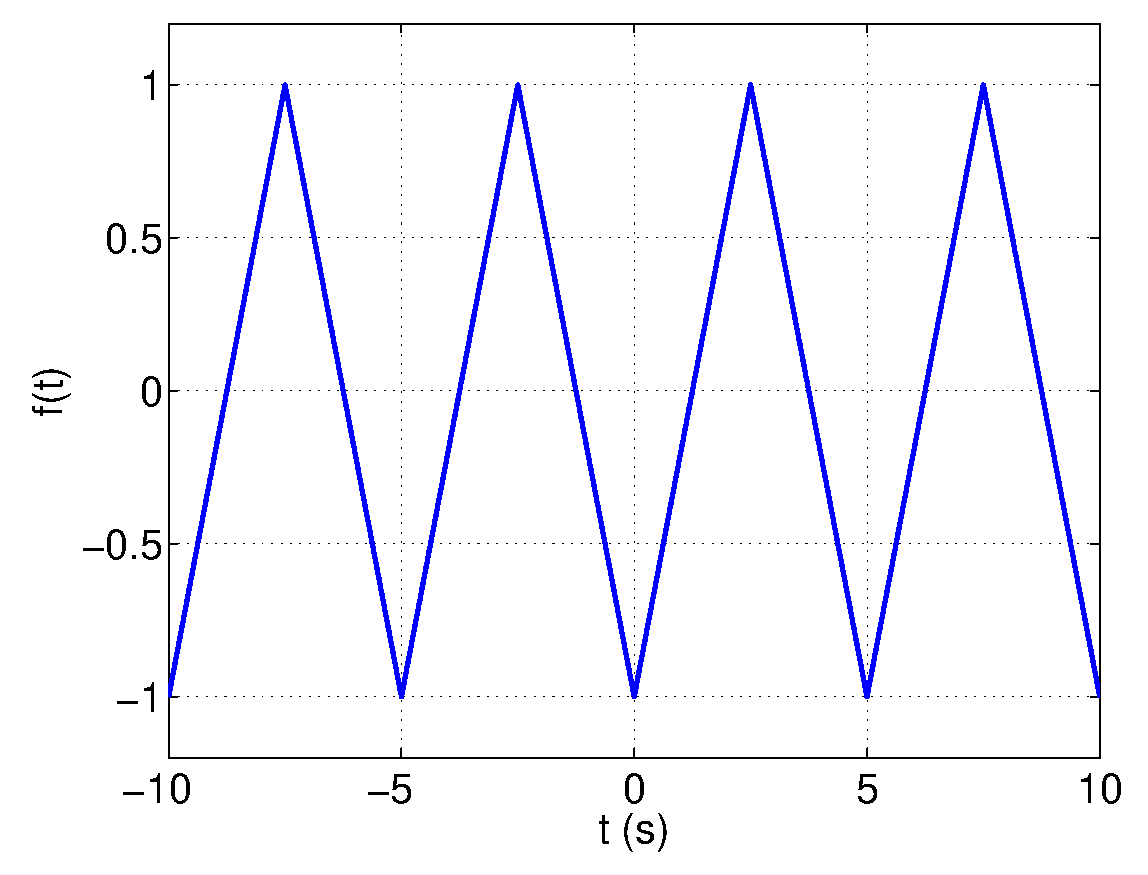
\includegraphics[width=4.5cm]{./Figuras/Triangular.eps} 

$T=5$
\end{figure}

    
    \end{column}
    \end{columns}


\end{itemize}

\end{frame}

\begin{frame}
\frametitle{Señales básicas: chirp  }

\begin{itemize}

\begin{columns}[c]

\hspace{-0.5cm}	\begin{column}{4.5cm}
    
        \item \alert{Chirp de variaci\'{o}n lineal}

\vspace{0.3cm}




\begin{figure}
    \centering
\footnotesize
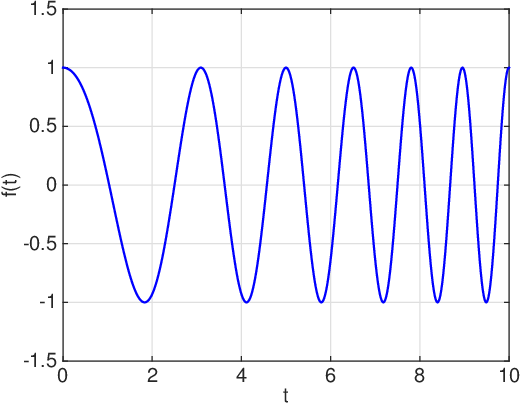
\includegraphics[width=4.5cm]{./Figuras/chirp} 

$f_{t=0}=0.2$ y $f_{t=10}=1$ 
\end{figure}

    
    \end{column}
    \end{columns}


\end{itemize}

\end{frame}

